%\documentclass{beamer}
%\usetheme{Pittsburgh} 
\documentclass{scrartcl}

\usepackage[utf8]{inputenc}
\usepackage{default}
\usepackage[procnames]{listings}
\usepackage{graphicx}
%\usepackage[toc,page]{appendix}
\usepackage{caption}
\usepackage{hyperref}
\usepackage{color}
\usepackage{pdfpages}


%Bibliogrpahy?
\usepackage{bibentry}
%\nobibliography*
%\bibentry{ }


\begin{document}

\title{Assignment No. 2}
\subtitle{}
\author{
  Quignon, Christophe \\
 Ali, Daiem(2-4)
  %Familyname, Name
} 
\date{\today}


\maketitle

\section{Read chapter 2 from Haykin’s book until 2.13 (leaving out Statistical learning theory to
end of chapter) and summarize or sketch your insights in mind-map or an outline or a
summary.
}
\begin{enumerate}
\item Introduction
	\begin{itemize}
	\item Learning from the environment and improving performance are key properties of a NN.
	\item The learning process has three major steps:
		\begin{itemize}
		\item stimulation of the NN
		\item change of the NN
		\item new respond of the NN
		\end{itemize}
	\end{itemize}
\item Error Correction Learning
	\begin{itemize}
	\item The error is defines ad the desired output - the actual output
	\item We want to minimize this error by adding costs to it. 
	\item This is called delta rule or Widrow-off rule.
	\item The adjustment of a neuron is proportional to the neurons input and error.
	\item To minimize the error, it must be observable.
	\item This proportion is denoted in the learning-rate parameter $\eta$ (eta)
	\item The tuning of $\eta$ is critical for a NN.
	\end{itemize}
\item Memory Based Learning
	\begin{itemize}
	\item Memory based learning involves:
		\begin{itemize}
		\item A criterion to define the local neighborhood to test against.
		\item A learning rule to be applied to the neighborhood
		\end{itemize}
		
	\item under certain circumstances (infinite sample size, identical and independent distribution), the error of the nearest neighbor is proven to be bounded to twice the bayesian probability of the error.
	\item The number of neighbors compared may vary.
	\item Outliers may be discarded.
	\end{itemize}
	
\item HEBBIAN Learning
	\begin{itemize}
	\item There are two major steps in hebbs learning:
		\begin{itemize}
			\item What fires together, wires together (enhancement)
			\item Neurons that are activated asynchronous, weaken their synapses. (depression)
		\end{itemize}
		\item From that we deduce four basic observations:
			\begin{itemize}
			\item Synaptic strengthening is time dependent
			\item It is dependent on the location of the neurons
			\item It is an interactive mechanism, because it takes neurons in front and after the the activated neurons in consideration
			\item It is a correlated mechanism, because the strengthening involves two. 
			\end{itemize}
		\item From Hebbian synapses, non-hebian and anti-hebian synapses are defined.
		\item Hebb's hypothesis may be varied with the learnig rate $\eta$
		\item It may furthe be improved by the covariance hypothesis with takes previous and following synaptic signals into consideration (averaged).
		\item This allow convergence and predicion of potentiation or depression
		\item The hippocampus is formed by hebbian learning. 
	\end{itemize}
	
\item Competitive learning
	\begin{itemize}
	\item In competitive learning, only one neuron is active at any time. The neurons compete to become this one active neuron.
	\item There are three basic elements to competitive learning:
		\begin{itemize}
		\item Weights are randomly distributed
		\item There is a limit to the strength of a neuron
		\item A mechanism to permit neuron activation, so only one neuron is active (winner takes it all)
		\end{itemize}
	\item To become a winner in a competitive learning NN, neurons become specialists: feature detectors.
	\item In a competitive learning NN, the neurons of one layer may be connected to inhibit their firing. (lateral inhibition)
	\item A neuron learns by shifting weights from inactive to active inputs
	\item A good example of competitive learning is clustering
	\end{itemize}
	
\item Boltzmann learning
	\begin{itemize}
	\item Boltzmann learning is inspired by statistical mechanics.
	\item The neurons activation is binary
	\item The network is defined by an energy function
	\item The activation of the neurons flip at random
	\item This flip changes the energy function and will end in a thermal equilibrium.
	\item The Boltzmann NN has two kinds of neurons:
		\begin{itemize}
		\item visible neurons which are the interface to the environment (may be fixed)
		\item hidden neurons who operate freely
		\end{itemize}
	\end{itemize}
	
\item Credit assignment problem
	\begin{itemize}
	\item The credit assignment problem is the task to divide the reward of a successful to the single components. (Same for unsuccessful)
	\item The problem is dependent on the time of the success (temporal credit-assignment)
	\item It is also concerned with the weighting of the success to the internal structure (structural credit assignment problem)
	\end{itemize}
	
\item Learning with a teacher
	\begin{itemize}
	\item A teacher already learned the desired output
	\item The difference between the teacher output (desired) and the output of the learning system is fed back
	\item The teacher is the optimum to reach
 	\end{itemize}
 	
\item Learning without teacher
	\begin{itemize}
	\item Without a teacher it is hard to find the error.
	\item A critic, who acknowledges good moves, is introduced
	\item In reinforcement learning the system can learn how to optimally approach a goal by delaying the reinforcement
	\item This includes the temporal credit assignment problem
	\item Reinforcement learning is closely related to dynamic programming.
	\item Unsupervised learning was neither a teacher nor a critic
	\item Unsupervised learning uses competitive neurons
	\end{itemize}
	
\item Learning tasks
	\begin{itemize}
	\item Pattern association may happen autoassociative (comparison to stored goal) or heteroassociative (input output pairs)
	\item In pattern recognition, inputs are put into classes by similarity
	\item Pattern recognition is split into feature extraction and classification
	\item Function approximation can be done with system identification  (memoryless MIMO) or with inverse system 
	\item Control can also efficiently be learned with a NN
	\item NN control can handle nonlinear noise and develop longtime plans
	\item Control learning may happen indirect with the systems in and output or direct with the signs of the partial derivatives
	\item Filtering of noise with filters, smoothing or prediction is a common field of NN learning
	\item Beamforming as a subfield of filtering because it copes with cut out beams of information from the environment
	\end{itemize}

\item Memory
	\begin{itemize}
	\item Characteristics:
		\begin{itemize}
		\item distributed
		\item both stimulus and response are stored 
		\item memory is resistant to noise
		\item interactions between patterns are also stored
		\end{itemize}
	\item The memory can be stored in memory matrix which contains the weight of all neuronal connections
	\item One fundamental function of the memory is to recall patterns
	\end{itemize}
	
\item Adaptation
	\begin{itemize}
	\item It is crucial to adapt behaviour with respect to the time
	\item Only non-static environments have a time component to which the NN has to adapt to.
	\item  However, some signals (speech, radar) are stationary over a certain period of time
	\item This pseudostationary property can be exploited (only use change, change monitoring time)
	\end{itemize}
\end{enumerate}

%\begin{itemize}
%\item
%\end{itemize}
\newpage

\section{Design a perceptron that computes the following Boolean function:
}
\subsection{f(x1 , x2 ) = NOT(x1 AND x2 )}

$b = w_{0} = -1.5$\\
$w_{1} = -1$\\
$w_{2} = -1$\\

\begin{tabular}{cc|c|c|c}
x1*-1 & x2*-1 & $\Sigma$ &$\geq$ -1.5 & $\neg(x1 \land x2)$\\\hline
0&0&0&1&1\\
0&-1&-1&1&1\\
-1&0&-1&1&1\\
-1&-1&-2&0&0
\end{tabular}


\subsection{f(x1 , x2 , x3) = (x1 AND x2 ) OR x3}
$b = w_{0} = 1.5$\\
$w_{1} = 1$\\
$w_{2} = 1$\\
$w_{3} = 2$\\

\begin{tabular}{ccc|c|c|c|c}
x1*1 & x2*1 & x3*2 &$\Sigma$ &$\geq$ 1.5 & $(x1 \land x2)\lor x3$\\\hline
0&0&0&	0&0&0\\
0&0&1&	2&1&1\\
0&1&0&	1&0&0\\
0&1&1&	3&1&1\\
1&0&0&	1&0&0\\
1&0&1&	3&1&1\\
1&1&0&	2&1&1\\
1&1&1&	4&1&1\\

\end{tabular}

\newpage
\section{}
\subsection{A basic limitation of the perceptron is that it cannot implement the EXCLUSIVE OR
function. Explain the reason for this limitation.}
In a graphical representation of the boolean function, the exclusive or requires two straight lines to separate true from false. A single linear perceptron however can only draw one straight line.

\subsection{Show that neural networks with one hidden layer can describe all Boolean functions.}
Since every Boolean function can be transformed into conjunctive normal form, we can design a neuronal network with negation as weights, the conjunctions at the first level and the disjunctions in the hidden layer. From that follows that every boolean function can be modeled in a two layer neuronal network.

\section{Let these networks be ADALINE. Derive the Delta rule for the following two networks.}
\subsection{}
$\Delta w_{kj}(n)=e_{k}(n)x_{j}(n)$\\
$\Delta w_{kj}(n)=(d_{k}(n)-y_{k}(n))x_{j}(n)$\\
$\Delta w_{0j}(n)=(d_{0}(n)-y_{0}(n))
(w_{0}+x_{1}w{1}+x_{2}w_{2})$\\

\subsection{}
$\Delta w_{kj}(n)=e_{k}(n)x_{j}(n)$\\

$\Delta w_{1j}(n)=(d_{1}(n)-y_{1}(n))x_{j}(n)$\\
$\Delta w_{1j}(n)=(d_{1}(n)-y_{1}(n))
(+x_{1}w{1}+x_{2}v_{1})$\\

$\Delta w_{2j}(n)=(d_{2}(n)-y_{2}(n))x_{j}(n)$\\
$\Delta w_{2j}(n)=(d_{2}(n)-y_{2}(n))
(x_{1}w{2}+x_{2}v_{2})$\\



$\Delta w_{3j}(n)=(d_{3}(n)-y_{3}(n))x_{j}(n)$\\
$\Delta w_{0j}(n)=(d_{0}(n)-y_{0}(n))
(y{1}u_{1}+y_{2}u_{2})$\\

\section{Do the problem 1.13 (Network architecture) from the previous week’s assignment.}
\subsection{This time use MATLAB or Python’s (sympy) symbolic toolbox. Finally assume the network
presented in fig P1.13 is a binary-classifier, please depict how the input space (R2) is classified
on a 2D graph using different colors.}

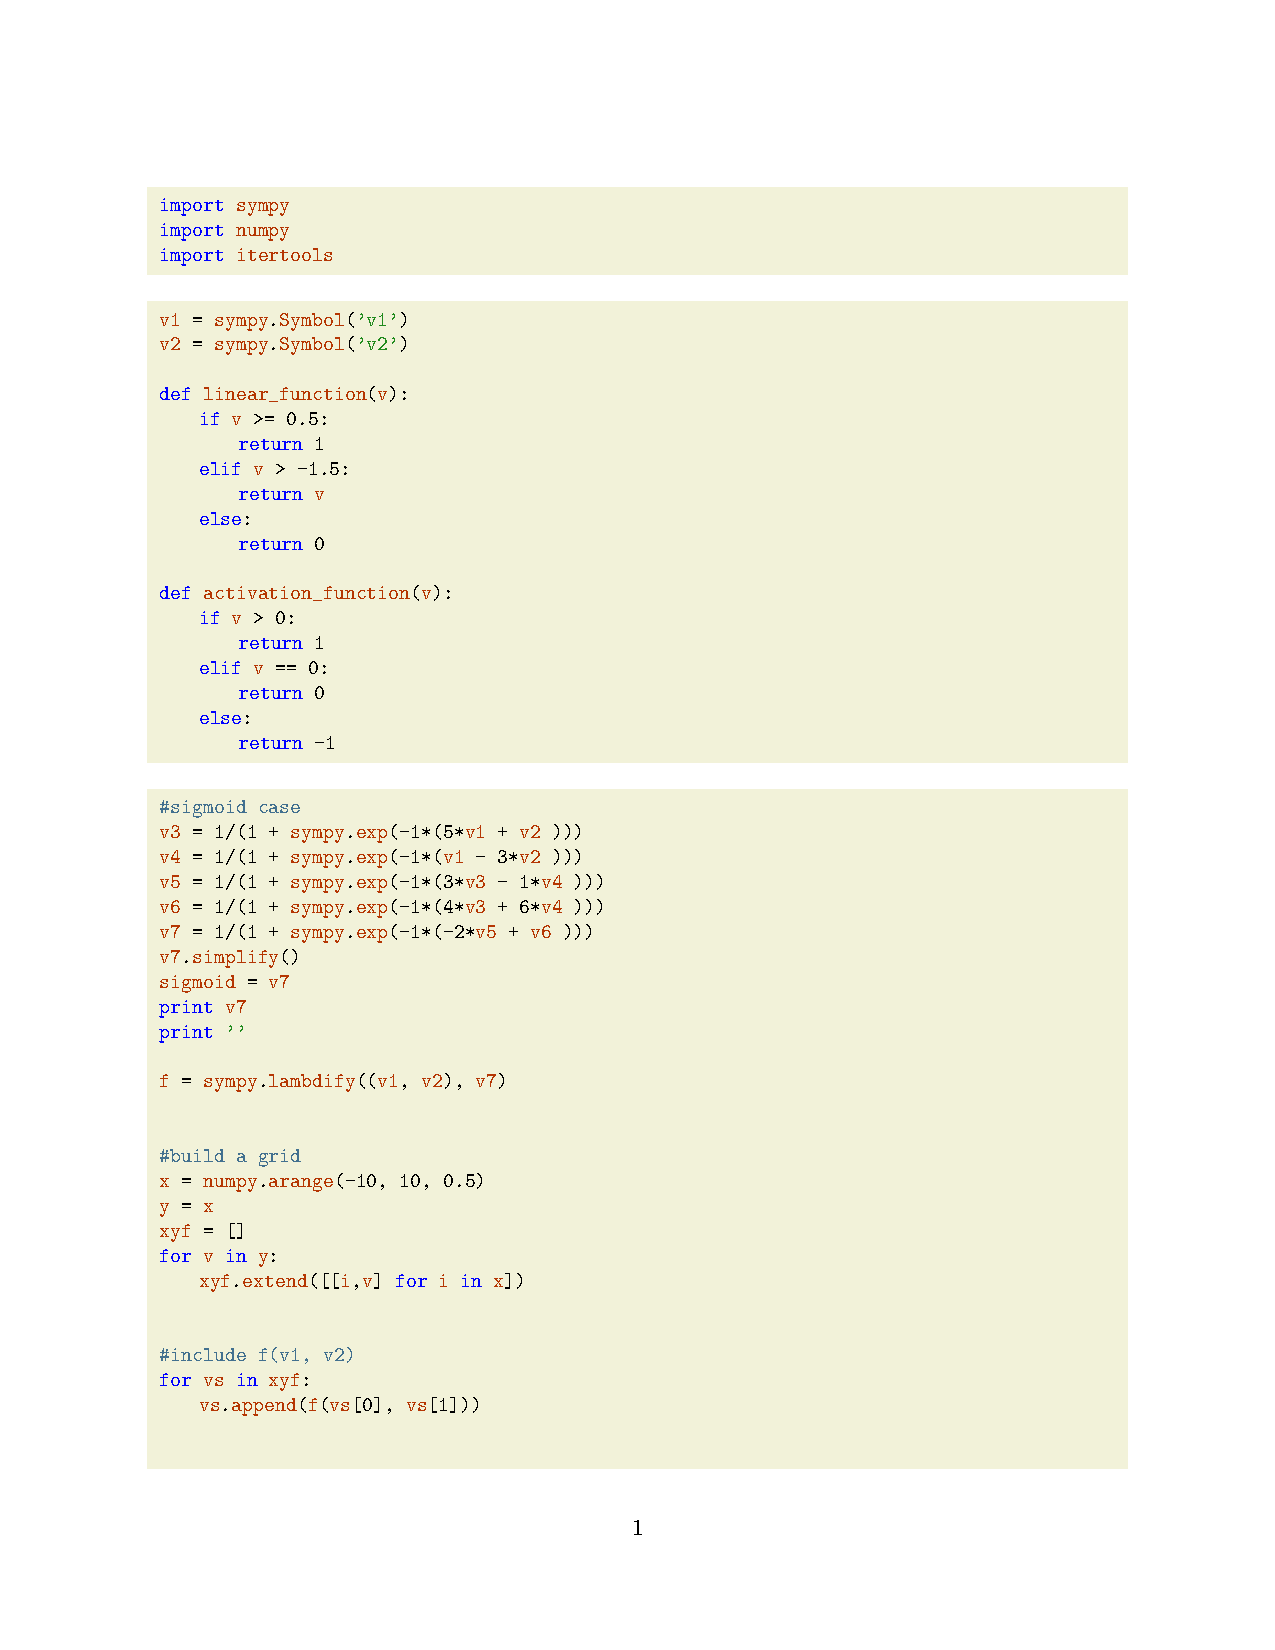
\includepdf[pages={1-},scale=1]{Neurons.pdf}

\subsection{Please upload 3 questions and their brief answers on the reading material in a separate txt
file.
}
See:  NN\_ChristopheQuignon\_131014.qqq


%CONTENTS
%NOTES


%COPY AND PASTE FROM HERE

%\begin{enumerate}
% \item 
%\end{enumerate}

%\hyperref{link}{text}

%\begin[Language=Python]{lstlisting}
%#PYTHON CODE HERE
%\end{lstlisting}

%\lstinputlisting[Language=Python]{ }

%\begin{figure}
% \center
% \includegraphics[width= cm]{ }
% \caption{}
%\end{figure}

%BIBLIOGRPAHY?
\bibliographystyle{plain}%amsalpha
\bibliography{Top30.bib}
%\bibentry{}

\end{document}
